{\let\clearpage\relax
\chapter{Termin- \& Ressourcenplanung}}
\label{sec:terminplanung}

\section{Terminplanung}
Eintacktung der Arbeitspakete in einen Terminplan.
\begin{figure}
	\centering
	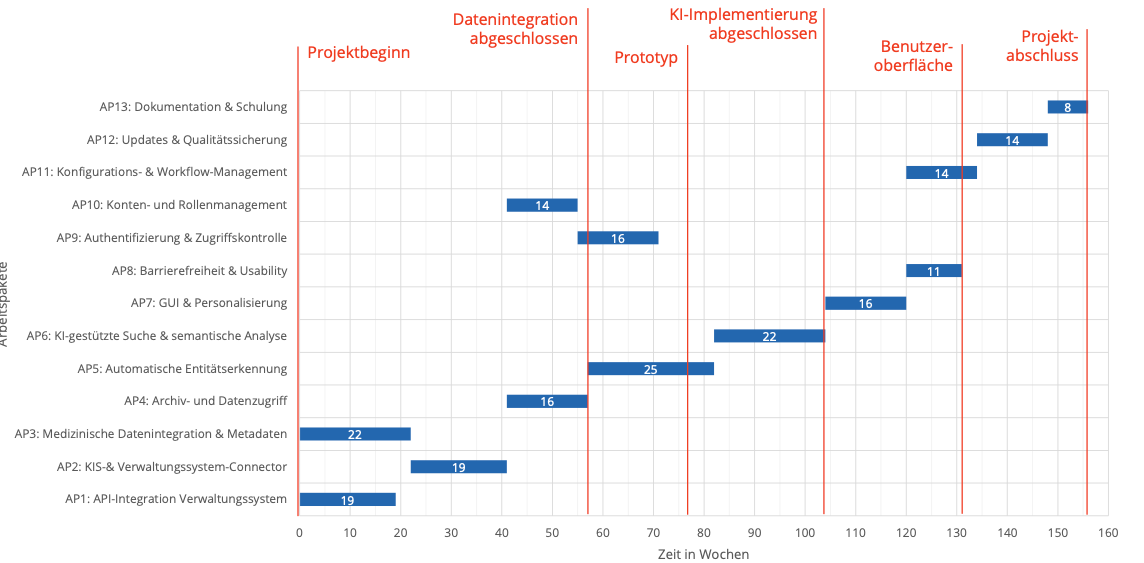
\includegraphics[width=0.9\textwidth]{fig/Terminplanung.png}
	\caption{Terminplanung - Tätigkeitsplan (Aufgaben stehen Zeitachse gegenüber)}
	\label{fig:terminplanung}
\end{figure}

\section{Ressourcenplanung}
\subsection{Personalplanung}
Den Arbeitspaketen werden die verschiedenen Personengruppen zugeordnet und ein bestmögliches szenario gesucht um möglichst effizient die Arbeitspakete zu bearbeiten.
\begin{center}
\begin{tabular}{p{2cm} p{4cm}|p{2cm} p{5cm}}
	BE & Backend- Entwicklung & DEVOPS & Architektur \& DevOps \\
	MI & Medizininformaik & SEC & IT-Sicherheit \\
	AI & KI/Data Science & UX & User Experience \\
	FE & Frontend & QA & Testautomatisierung \& QA \\
	TE & Tester & PJ & Projektleiter \\
	SH & Stakeholder & DE & Data Engineer \\
	BA & Dusiness Analyst & TR & Technische Redaktion
\end{tabular}
\end{center}

Durch analysieren verschiedener möglichen Szenarien und zusammenschluss von Parallel ausführbaren Arbeitspaketen ergibt sich folgende Einteilung:
\begin{figure}[ht]
	\centering
	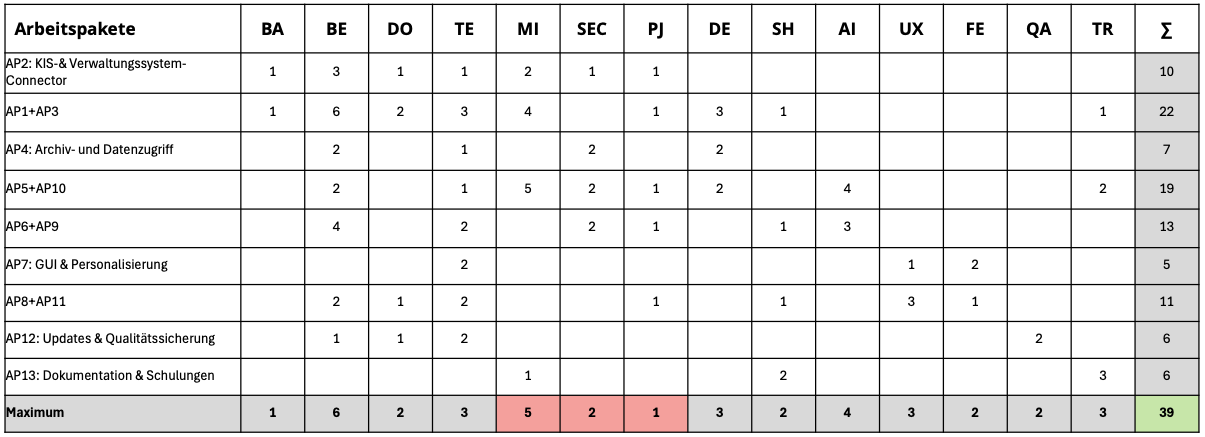
\includegraphics[width=0.9\textwidth]{fig/arbeiter.png}
	\caption{Mitarbeiterverteilung auf die Arbeitspakete}
	\label{fig:arbeiter}
\end{figure}
\subsection{Sachmittelplanung}
Jede Aufgabe braucht gewisse Arbeitsmaterialien um abgeschlossen zu werden. Dazu findet sich hier die Planung der verschiedenen Sachmittel.

\begin{figure}[ht]
	\centering
	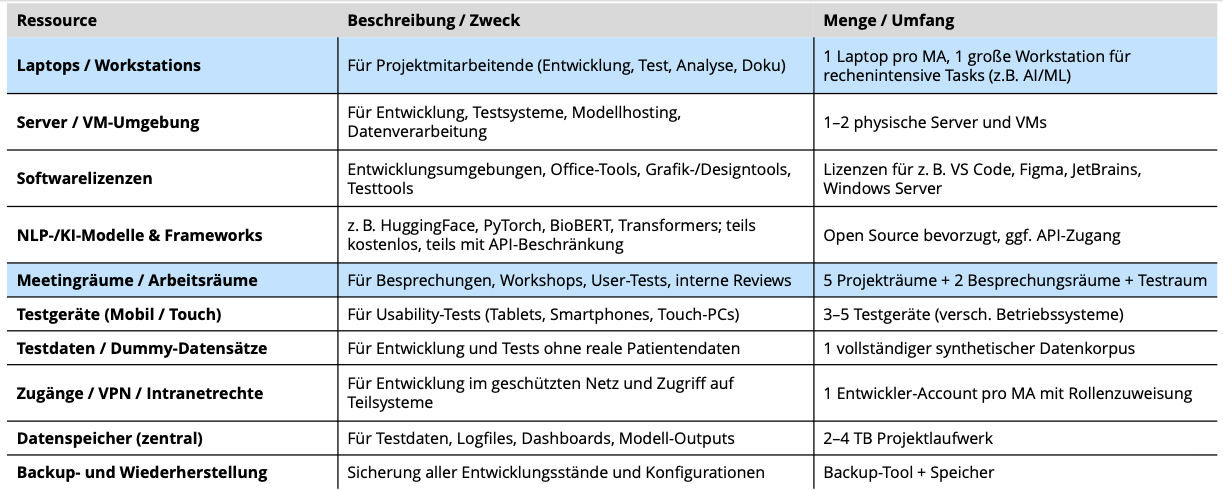
\includegraphics[width=0.9\textwidth]{fig/material.png}
	\caption{Benötigte Arbeitsmaterialien}
	\label{fig:material}
\end{figure}\begin{figure}
	\centering
	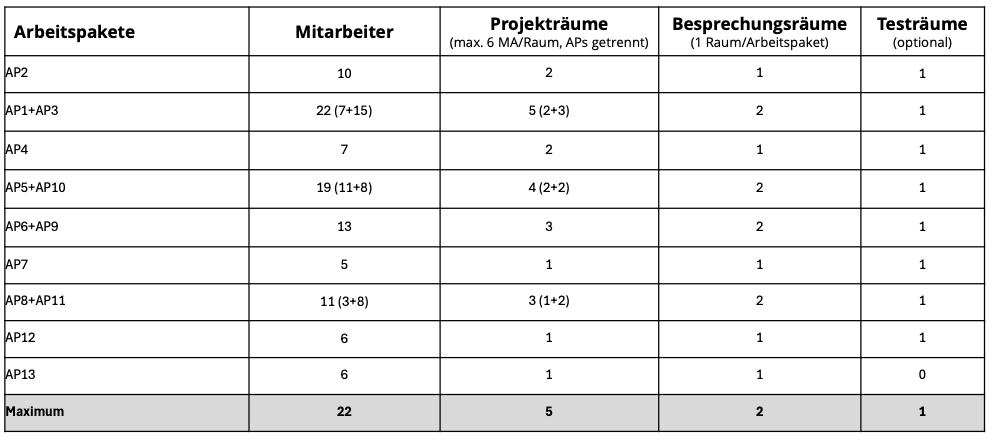
\includegraphics[width=0.9\textwidth]{fig/räume.png}
	\caption{Benötigte Räumlichkeiten}
	\label{fig:räume}
\end{figure}